\section{Análise de sentimentos de coonsumo e político (GODSentimentAnalysis)}

\textbf{Grupo:}\textit{Ana Luisa de Almeida Losnak, Arthur Branco Costa, Daniel Costa Bucher, Diego de Araújo Martinez Camarinha, Rafael Batista Carmo}

\textbf{Contato:}analosnak@gmail.com


\subsection{Introdução}
GOD Project é um sistema desenvolvido em \texttt{Smalltalk} que captura dados de diversas fontes da internet, como páginas web e redes sociais. GOD processa esses dados e fornece informações para diferentes aplicações.

Nosso grupo ficou responsável pelo desenvolvimento das seguintes aplicações:

\begin{itemize}
	\item Análise de Sentimento de Consumo:
	
	Aplicação na qual o usuário faz uma busca por determinado produto, e o GOD devolve as estatísticas a respeito dele, no formato desejado (planilha ou gráfico).
	
	Nos resultados são mostrados quantas postagens nas redes sociais foram a favor, contra e neutras a respeito desse produto.
	
	\item Análise de Sentimento Político:
	
	Nesta aplicação a busca consiste em dois campos: o nome de um candidato e seu partido político. É possível ainda procurar apenas pelo partido e ver as opiniões sobre ele de um modo geral.

	Também indica-se o formato de saída desejado (planilha ou gráfico) e após apertar o botão ``Go'', a pesquisa inicia-se.
\end{itemize}


A seguir listamos as classes que criamos (nos pacotes GODSentimentAnalysis e GODSentimentAnalysisTests) e redigimos um breve descrição sobre cada um dos seus principais métodos, tanto os de classe quanto os de instância. A saber suas diferenças:

Métodos de instância operam em objetos e conseguem acessar, processar e até modificar o estado do objeto tratado; em contrapartida, ainda que métodos de classe operem sobre a classe como um todo e também possa modificar atributos de classe, eles não têm acesso a variáveis de uma instância em particular. Em \texttt{Smalltalk}, métodos de classe correspondem a mensagens para o objeto representativo da classe, ao passo que métodos de instância correspondem a mensagens enviadas para um determinado objeto da classe em questão.

\subsection{SAInterface}
Classe principal que chama todas as outras, deve ser a única utilizada por outros pacotes. Ou seja, é a única classe que seria pública.

\texttt{analyse: as:} é o método principal de toda a aplicação, o único método de instância dessa classe e que deve ser chamado pelo usuário do pacote.

Além do analyse, ela possui mais cinco métodos de classe, todos eles responsáveis pela criação dos dicionários de termos positivos e negativos:

\subsubsection{Léxicos de Sentimento}
Todas as palavras dos dicionários desta classe foram retiradas do \textbf{OpLexicon}, um léxico de sentimento para a língua portuguesa, do OntoLP, um portal de ontologias.

Após baixarmos esse léxico tivemos que tratá-lo para adequá-lo melhor ao GOD, fazendo as seguintes alterações:

\begin{itemize}

	\item Remoção dos verbos:
	Os verbos dessa lista constavam apenas no infinitivo. Para sua utilização de forma eficiente, seria necessário incluir suas conjugações mais utilizadas.
	
	\item Português brasileiro:
	As palavras lá listadas estavam em português de Portugal, então tivemos que realizar modificações para o português brasileiro, tais como: género - gênero; projecto - projeto; tónico - tônico, etc.
	
\end{itemize}

\subsection{SAFetcher}
Devolve postagens relevantes da rede social escolhida (Twitter ou Facebook) que contenham o termo pesquisado, no caso um \texttt{tag}.

O método \texttt{getTweets} pega no máximo cem tweets (limitação da API) da classe SNETTwitterFetcher

O método \texttt{setSession} auxilia a correta implementação dos testes utilizando mock.

\subsection{CSAApp}
Estas classes são responsáveis por manter o conteúdo HTML da página Web da aplicação de Análise de Consumo.

\texttt{renderResponse}: este método faz a validação dos dados inseridos pelo usuário. Apenas verifica se o campo do produto não está vazio.

Os demais métodos de instância incluem: inicialização, renderização da tela do navegador e o \texttt{save} que retorna os valores de um formulário.

\subsection{PSAApp}
Classes análogas às anteriores, porém tratam sobre a Análise de Sentimento Político. Os métodos adicionais da \texttt{PSAApp} lidam com a validação dos dados retirados do TSE.

\texttt{validateCandidates} e \texttt{validateCandidates:using:} valida a entrada do usuário, verificando se o candidato está em alguma das listas de cargo (presidente, governador, senador, etc). Por último o método \texttt{validateParty}, que verifica se o partido está na lista de partidos válidos.

\subsection{PSAPoliticalDataLoader}
No pacote \texttt{accessor} encontram-se métodos que servem apenas para retornar os dicionários de candidatos por cargo, partidos e UFs. Já no pacote \texttt{initializer} localizam-se os métodos que buscam os candidatos por cargo e estado no site do TSE.

\subsection{SAApp}
Classe que cria e preenche a estrutura de dados desejada para ser apresentado na Web. Se o usuário escolhe ``planilha'', esta classe que se comunica com a WEBSpreadSheet e formata como deve ser a planilha, no fim das contas. O mesmo ocorre quando o parâmetro passado é ``Grafo''.

\subsection{SAOutputGenerator}
Esta classe é responsável por gerar um grafo ou uma planilha a partir dos resultados e avaliações das pesquisas sobre análise de sentimento recebidas, dependendo da escolha do usuário (\texttt{generateGraph:} e \texttt{generateSpreadsheet:}) e exporta o que foi gerado (\texttt{export:as:}).

\subsection{SASentimentAnalyser}
Nesta classe, ocorre a classificação das opiniões retiradas das redes sociais através da utilização dos dicionários de palavras positivas e negativas. Por enquanto, o único critério adotado foi a contagem de cada tipo de palavra. Por exemplo, se há mais palavras positivas na postagem, ela inteira será contabilizada como positiva.

Contudo, após essa contagem e analisada a proporção entre os dois tipos de palavras, é calculado ainda um viés. Se a diferença entre palavras positivas e negativas for menor que um índice que escolhemos, o texto é classificado como neutro.

\subsection{SASentimentLabel}
\texttt{SASentimentLabel} nada mais é do que uma classe para armazenar e retornar os tipos possíveis de classificação (GOOD, BAD ou NEUTRAL).

\subsection{SASentimentTable}
Esta classe é responsável por fazer uma tabela de sentimentos (GOOD, BAD ou NEUTRAL). Ela leva em consideração as avaliações feitas.

\subsection{UML}
Afim de esclarecer ainda mais as coisas, optamos por fazer um diagrama UML para facilitar a compreensão da  modelagem adotada por nosa equipe. A seguir pode-se observar a relação entre as classes, bem como todos os seus métodos que listamos anteriormente e ainda, é possível conferir os parâmetros passados e seus tipos, bem como o tipo de retorno de cada função.

\begin{figure}[h]
\caption{Diagrama UML}
\centering
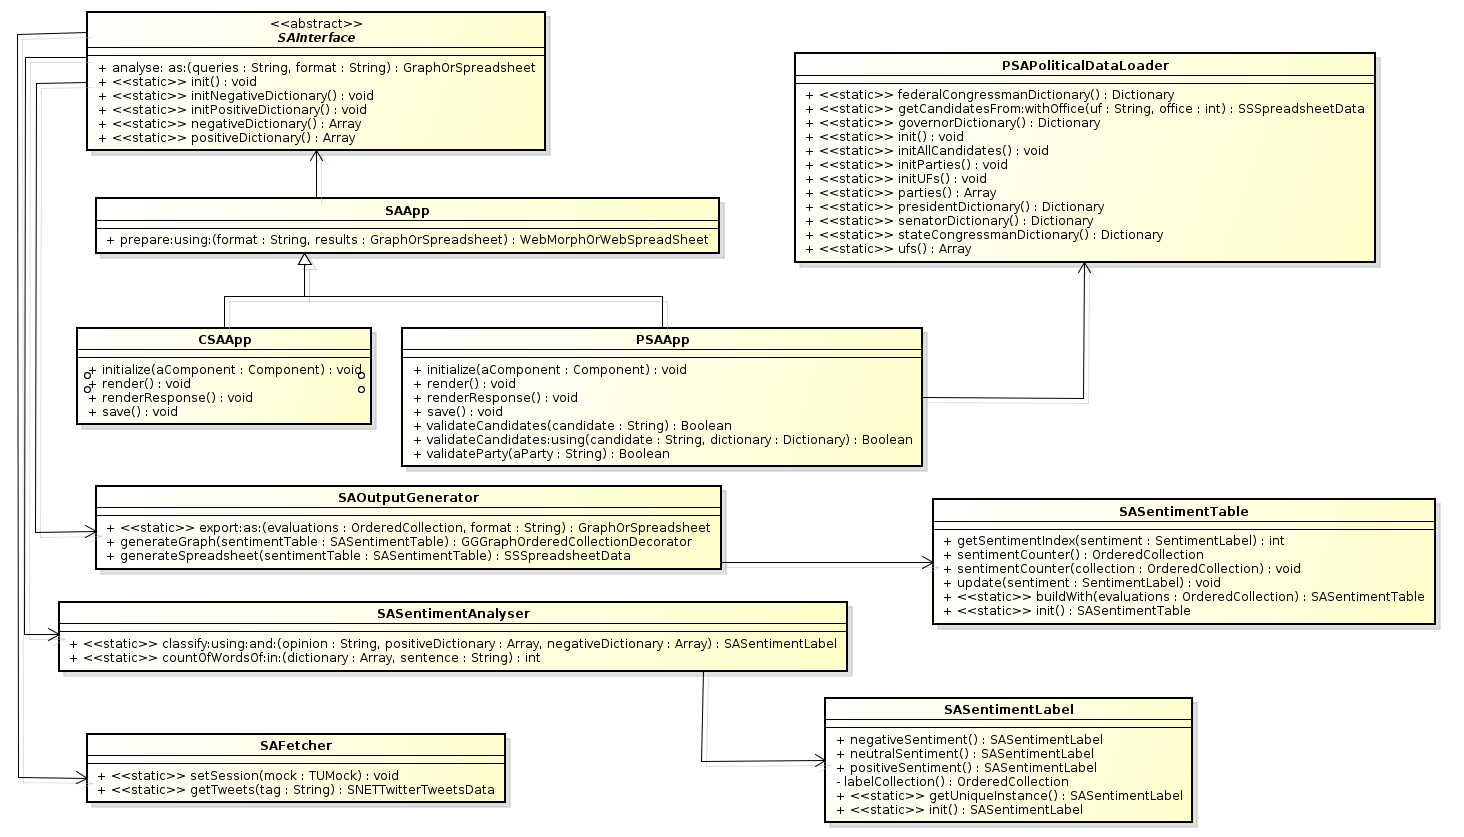
\includegraphics[width=16cm]{figures/UML.png}
\label{fig:uml}
\end{figure}

\newpage
\subsection{Rodando as Aplicações}
Para iniciar as aplicações de Análise de Sentimento basta seguir o simples passo-a-passo abaixo:

\begin{enumerate}
	\item No Squeak, abrir o Seaside Control Panel
	
	\item Dentro dele, clicar com o botão direito e então na opção Add adaptor...
	
	\item Escolher o tipo: WAComancheAdaptor
	
	\item Pressionar o botão ``Start''
	
	\item Abrir o navegador no endereço: localhost:8080/god
\end{enumerate}

Feito isso aparecerá a tela inicial, figura \ref{fig:ini}.

\begin{figure}[h]
\caption{Tela Inicial}
\centering
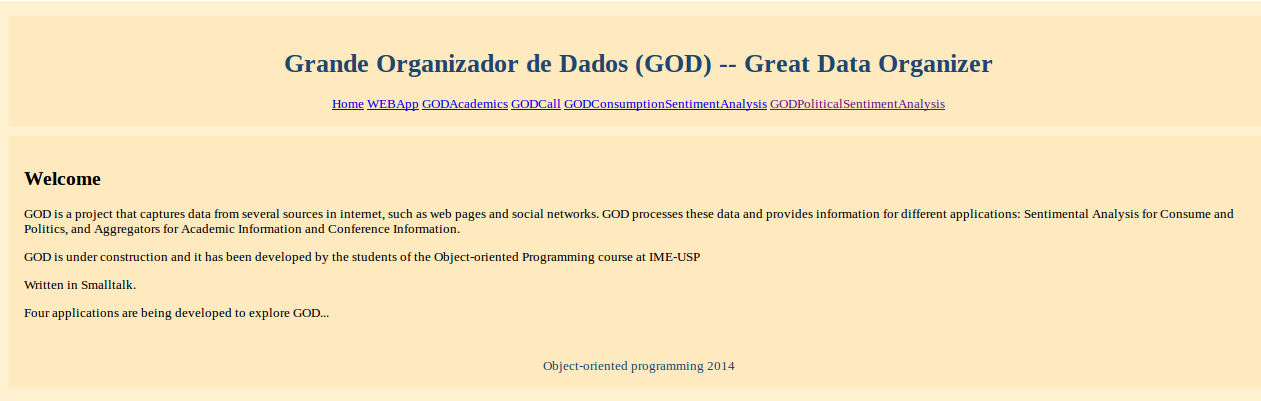
\includegraphics[width=14cm]{figures/inicio.png}
\label{fig:ini}
\end{figure}

\subsubsection{Análise de Sentimento de Consumo}
Para iniciar essa aplicação, basta clicar na opção do cabeçalho GODConsumptionSentimentAnalysis, que então surgirá a tela para pesquisar algum produto, figura \ref{fig:cons-pesq}.

\begin{figure}[h]
\caption{Análise de Sentimento de Consumo}
\centering
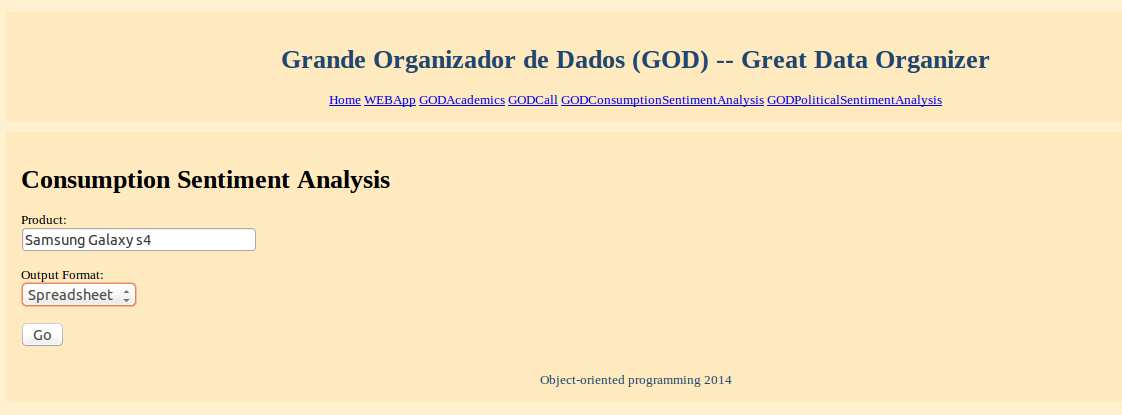
\includegraphics[width=14cm]{figures/consumo-pesquisa.png}
\label{fig:cons-pesq}
\end{figure}

Um possível resultado dessa pesquisa seria, por exemplo, o da figura \ref{fig:cons-result}, mostrado a seguir:

\begin{figure}[h]
\caption{Pesquisa - Galaxy s4}
\centering
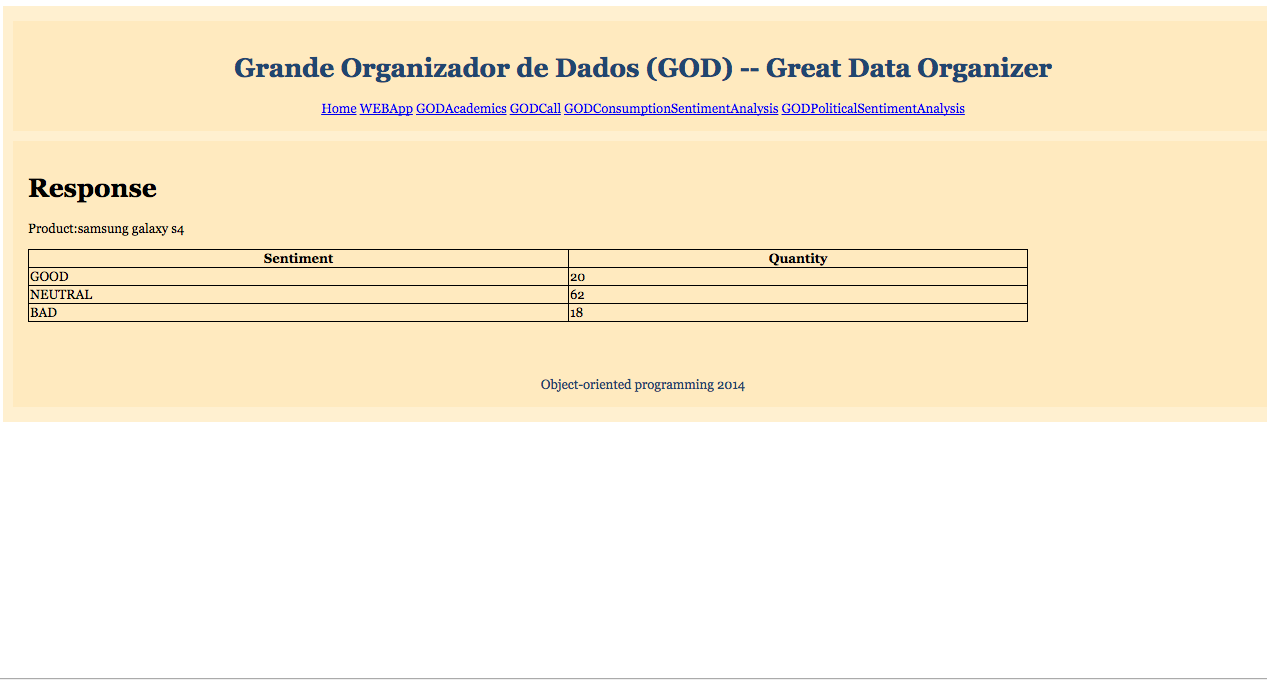
\includegraphics[width=14cm]{figures/consumo-resultado.png}
\label{fig:cons-result}
\end{figure}

\subsubsection{Análise de Sentimento de Político}
Para rodar essa aplicação é preciso selecionar a opção: GODPoliticalSentimentAnalysis, no cabeçalho. Assim, aparecerá a seguinte tela:

\begin{figure}[h]
\caption{Análise de Sentimento Político}
\centering
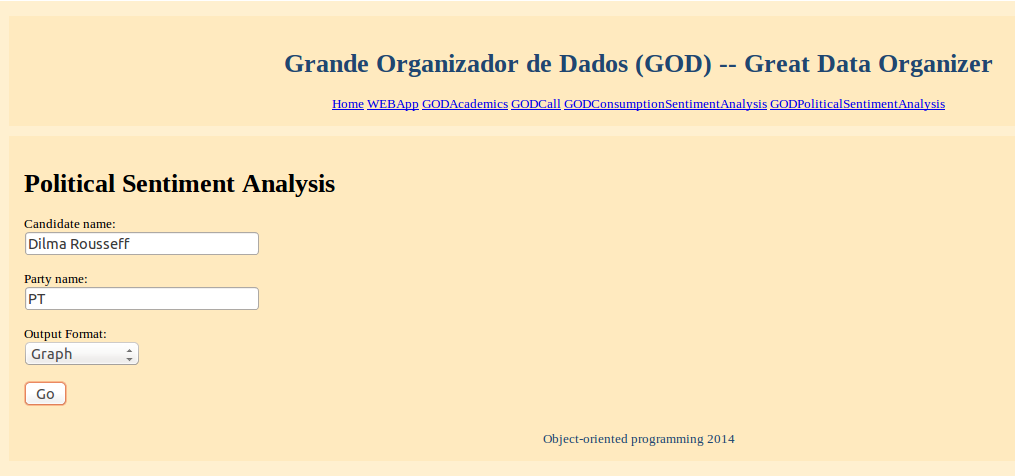
\includegraphics[width=14cm]{figures/politico-pesquisa.png}
\label{fig:pol-pesq}
\end{figure}

Um possível resultado dessa pesquisa seria, por exemplo, o da figura \ref{fig:pol-result}, mostrado a seguir:

\begin{figure}[h]
\caption{Pesquisa - Dilma PT}
\centering
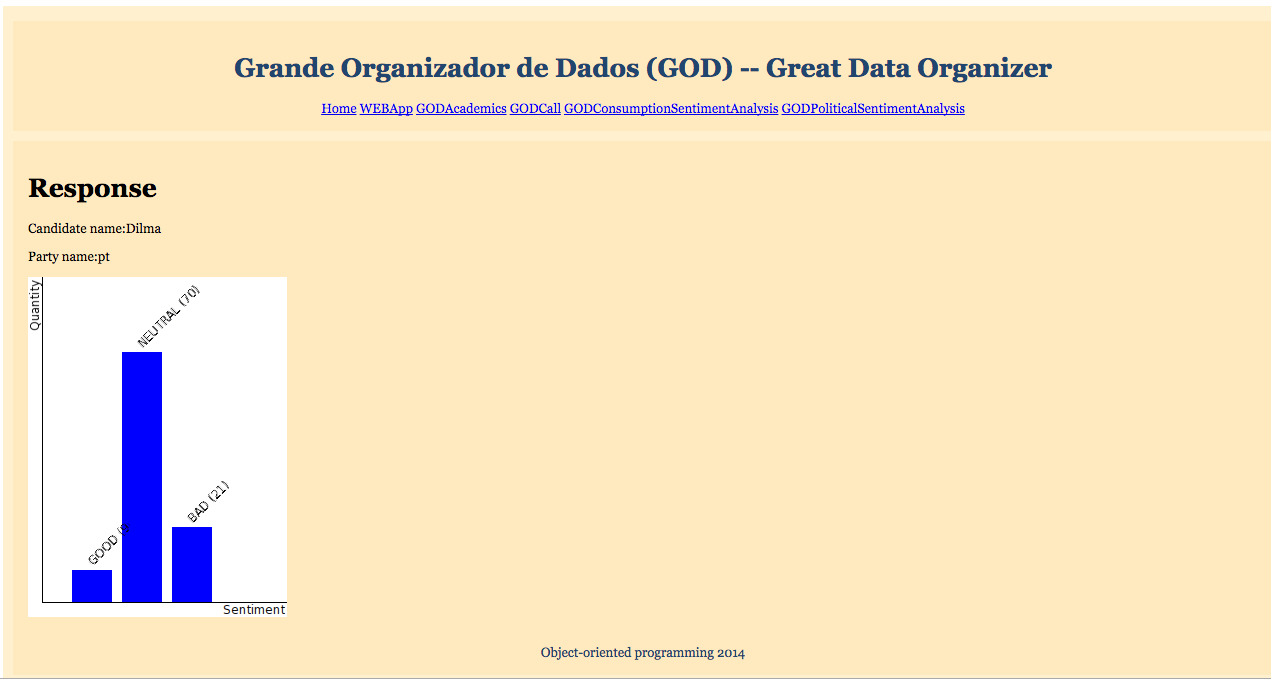
\includegraphics[width=14cm]{figures/politico-resultado.png}
\label{fig:pol-result}
\end{figure}
